% {{{ Preamble ----------------------------------------------------------------
\documentclass{beamer}

% encodings, fonts etc.
\usepackage[utf8x]{inputenc}
\usepackage[T1]{fontenc}

% Hold kæft utf
\makeatletter
\def\UTFviii@defined#1{%
  \ifx#1\relax
      ?%
  \else\expandafter
    #1%
  \fi
}

\makeatother

% math packages
\usepackage{amsmath, amssymb, amsthm}
\usepackage{mathtools}

% beamer configuration
\usetheme{Copenhagen}
%\usetheme{metropolis}
\beamertemplatenavigationsymbolsempty
%\setbeamertemplate{theorems}[numbered]
\setbeamersize{description width=2.0em}

%\usepackage{pgfpages}
%\setbeameroption{show notes}
%\setbeameroption{show notes on second screen=right}

% algorithms
\usepackage{algorithm}
\usepackage[noend]{algpseudocode}

% misc. packages
\usepackage{float}
\usepackage{varwidth}
\usepackage{listings}
\lstset{
  %breaklines=true,
  keepspaces=true,
  %frame=ltrb,
  %framesep=1pt,
  %commentstyle=\color{grey},
  basicstyle=\ttfamily\tiny,
  %numbers=left,
  title=\lstname,
  %columns=fullflexible,
  inputencoding=utf8,
  extendedchars=true,
}

% graphics and tikz
\usepackage{pgf}
\usepackage{tikz}
\usetikzlibrary{positioning,arrows,calc}
\tikzset{
    on grid,
    node distance=3cm,
    auto,
    block/.style = {
        draw,
        shape=rectangle,
        minimum height=3em,
        minimum width=3em,
        line width=1pt
    },
    control/.style = {
        draw,
        shape=circle,
        minimum height=7em,
        minimum width=3em,
        line width=1pt
    },
    mux/.style = {
        draw,
        shape=rectangle,
        minimum height=1.5em,
        minimum width=1em,
        line width=1pt
    },
    empty/.style = {
        shape=rectangle,
        minimum height=3em,
        minimum width=3em
    },
    >=latex',
}


% mathematics
\newtheorem{proposition}{Proposition}

\renewcommand{\tt}{\texttt}

% title page
\title{Core Components}
\author[Carl-Johannes Johnsen]{
  \mbox{Carl-Johannes Johnsen}}
\institute{Department of Computer Science\\
           University of Copenhagen}
%\date{December 22, 2016}
% }}} -------------------------------------------------------------------------

\begin{document}

% {{{ Title page --------------------------------------------------------------
\frame{\titlepage}
% }}} -------------------------------------------------------------------------

% {{{ Table of contents -------------------------------------------------------
%\begin{frame}
%  \frametitle{Outline}
%  \tableofcontents
%\end{frame}
% }}} -------------------------------------------------------------------------

\section{Introduction}
\begin{frame}
    In this lecture, we will be looking at the major components of the MIPS
    processor.

    \vspace{\baselineskip}
    By combining these components, we should be able to construct a single
    cycle MIPS processor.
\end{frame}
\subsection{Overview}
\begin{frame}
    \begin{figure}
        \centering
        \scalebox{0.5}{
            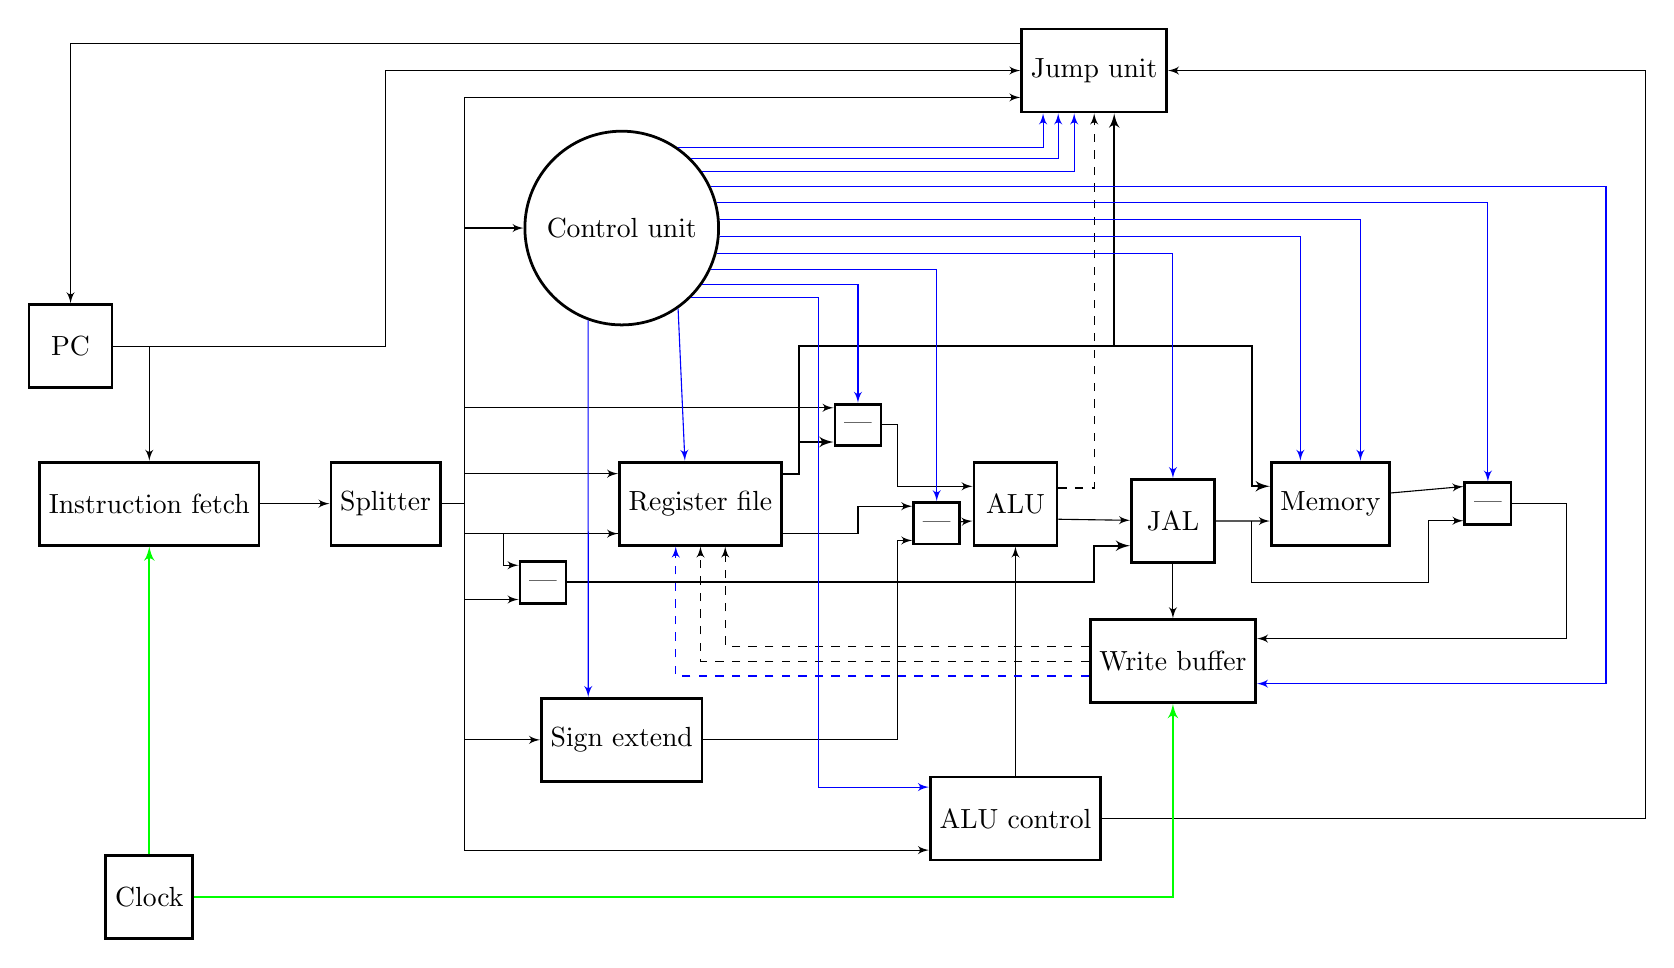
\begin{tikzpicture}
                \node[block] (reg) at (0,0) {Register file};
                \node[control] (cont) at (-1,3.5) {Control unit};
                \node[block] (jump) at (5,5.5) {Jump unit};
                \node[empty] (splitspace) at (-3,0) {};
                \node[block] (split) at (-4,0) {Splitter};
                \node[block] (if) at (-7,0) {Instruction fetch};
                \node[block] (sign) at (-1,-3) {Sign extend};
                \node[block] (alu) at (4,0) {ALU};
                \node[block] (alucont) at (4,-4) {ALU control};
                \node[block] (mem) at (8,0) {Memory};
                \node[block] (jal) at (6,-0.22) {JAL};
                \node[mux] (memread) at (10,0) {|};
                \node[mux] (shmt) at (2,1) {|};
                \node[mux] (imm) at (3, -0.25) {|};
                \node[mux] (regdst) at (-2,-1) {|};
                \node[block] (pc) at (-8, 2) {PC};
                \node[block] (writebuf) at (6, -2) {Write buffer};

                \path[draw, ->] (if) -- (split);
                \path[draw, -] (split) -- (splitspace.center);
                \path[draw, ->] (splitspace.center) |- (sign);
                \path[draw, ->] (splitspace.center) |- (cont);
                \path[draw, ->] (splitspace.center) |- (reg.160);
                \path[draw, ->] (splitspace.center) |- (reg.200);
                \path[draw, ->] (splitspace.center) |- (jump.200);
                \path[draw, ->] (splitspace.center) |- (alucont.200);
                \path[draw, ->] (splitspace.center) |- (regdst.215);
                \path[draw, ->] (splitspace.center) |- (shmt.145);
                \path[draw, ->] (reg.200) -| (-2.5, -0.5) |- (regdst.145);
                \path[draw, ->] (alucont) -- (alu);
                \path[draw, ->] (alucont) -| (12, 0) |- (jump);
                \path[draw, ->] (reg.340) -| (2,-0.25) |- (imm.145);
                \path[draw, thick, ->] (reg.20) -| (1.25,0.5) |- (shmt.215);
                \path[draw, thick, ->] (1.25, 0.5) |- (4, 2) -| (7,1) |- (mem.164);
                \path[draw, thick, ->] (4,2) -| (jump.295);
                \path[draw, ->] (shmt) -| (2.5, 0.5) |- (alu.158);
                \path[draw, dashed, ->] (alu.20) -| (jump);
                \path[draw, ->] (alu.340) -- (jal);
                \path[draw, ->] (jal) -- (mem.196);
                \path[draw, ->] (imm) -- (alu.202);
                \path[draw, ->] (7, -0.22) |- (8, -1) -| (9.25,-0.5) |-
                (memread.215);
                \path[draw, ->] (mem.10) -- (memread.145);
                \path[draw, ->] (sign) -| (2.5, -1) |- (imm.215);
                \path[draw, thick, ->] (regdst) -| (5, -0.6) |- (jal.210);
                \path[draw, ->] (pc) -| (if);
                \path[draw, ->] (pc) -| (-4, 4) |- (jump);
                \path[draw, ->] (jump.160) -| (pc);
                \path[draw, ->] (jal) -- (writebuf);
                \path[draw, ->] (memread) -| (11, -1) |- (writebuf.15);
                \path[draw, dashed, ->] (writebuf.170) -| (reg.300);
                \path[draw, dashed, ->] (writebuf) -| (reg);
                \path[draw, dashed, ->, color=blue] (writebuf.190) -| (reg.240);

                \path[draw, ->, color=blue] (cont.55) -| (jump.220);
                \path[draw, ->, color=blue] (cont.45) -| (jump.230);
                \path[draw, ->, color=blue] (cont.35) -| (jump.245);
                \path[draw, ->, color=blue] (cont.25) -| (11.5,0) |-
                (writebuf.345);
                \path[draw, ->, color=blue] (cont.15) -| (memread);
                \path[draw, ->, color=blue] (cont.5) -| (mem.55);
                \path[draw, ->, color=blue] (cont.355) -| (mem.125);
                \path[draw, ->, color=blue] (cont.345) -| (jal);
                \path[draw, ->, color=blue] (cont.335) -| (imm);
                \path[draw, ->, color=blue] (cont.325) -| (shmt);
                \path[draw, ->, color=blue] (cont.315) -| (1.5, 0.5) |-
                (alucont.160);
                %\path[draw, ->, color=blue] (cont.315) -- (reg.95);
                \path[draw, ->, color=blue] (cont.305) -- (reg.110);
                \path[draw, ->, color=blue] (cont.250) -- (sign.128);

                \node[block] (clock) at (-7, -5) {Clock};
                \path[draw, ->, thick, color=green] (clock) -- (if);
                \path[draw, ->, thick, color=green] (clock) -| (writebuf);
            \end{tikzpicture}
        }
    \end{figure}
\end{frame}


% exit section
\AtBeginSection{}
\section*{}

% {{{ Bibliography ------------------------------------------------------------
%\begin{frame}{Bibliography}
%  \tiny
%  \bibliographystyle{plain}
%  \bibliography{pl}
%\end{frame}
% }}} -------------------------------------------------------------------------

\end{document}
